\documentclass[a4paper,11pt]{article}
\usepackage{a4wide}%

\usepackage{fullpage}%
\usepackage[T1]{fontenc}%
\usepackage[utf8]{inputenc}%
\usepackage[main=francais,english]{babel}%

\usepackage{graphicx}%
\usepackage{xspace}%
\usepackage{float}

\usepackage{url} \urlstyle{sf}%
\DeclareUrlCommand\email{\urlstyle{sf}}%

\usepackage{mathpazo}%
\let\bfseriesaux=\bfseries%
\renewcommand{\bfseries}{\sffamily\bfseriesaux}

\newenvironment{keywords}%
{\description\item[Mots-clés.]}%
{\enddescription}


\newenvironment{remarque}%
{\description\item[Remarque.]\sl}%
{\enddescription}

\font\manual=manfnt
\newcommand{\dbend}{{\manual\char127}}

\newenvironment{attention}%
{\description\item[\dbend]\sl}%
{\enddescription}

\usepackage{listings}%

\lstset{%
  basicstyle=\sffamily,%
  columns=fullflexible,%
  language=c,%
  frame=lb,%
  frameround=fftf,%
}%

\lstMakeShortInline{|}

\parskip=0.5\baselineskip

\sloppy

%opening
\title{PROG2: Inversion de matrices}
\author{Rémi Hutin \and Rémy Sun}
\date{26 février 2016}


\begin{document}

\maketitle

\begin{abstract}

\end{abstract}

\section{Implémentation de matrices}

\subsection{Définition}

On définit une classe \texttt{Matrix} possédant trois champs privés : \texttt{size\_i} contenant le nombre de lignes de la matrice, \texttt{size\_j} donnant le nombre de colonnes et
 \texttt{contents} correspondant à la matrice des valeurs de la matrice à proprement dit.

Le champ  \texttt{contents}  contient un double vecteur de \texttt{scalar\_t} représenter la matrice des valeurs.

\subsection{Méthodes et fonctions}

On définit les méthodes publiques suivantes:

\begin{itemize}
\item \texttt{get\_size\_i} et \texttt{get\_size\_j} permettent de consulter la valeur des \texttt{size\_i} et \texttt{size\_j}
\item \texttt{set(j,j,x)} permet de remplacer la valeur d'indice \texttt{(i,j)} dans la matrice par \texttt{x}.\texttt{get(i,j)} permet de consulter la valeur d'indice\texttt{(i,j)} dans la matrice. \texttt{print()} affiche la matrice dans le terminal en formattant correctement l'affichage.
\end{itemize}

De plus, on définit en plus les fonctions suivantes:

\begin{itemize}
\item Des opérateurs \texttt{+},\texttt{-} qui effectuent la somme et la différence de deux matrices en effectuant un simple parcours de la matrice. Un opérateur \texttt{*} qui posséde deux sens différents: si le premier argument est un \texttt{scalar\_t} alors on effectue juste la mutltiplication scalaire de la matrice comme pour les opérateurs précédents. Si c'est une matrice, on effectue une multiplication matricielle.
\item Une fonction \texttt{transpose} qui crée la matrice transposée par simple parcours des valeurs de la matrice. Une fonction \texttt{Id} qui crée une matrice identité.
\item Une fonction \texttt{submatrix} qui crée explicitement la sous-matrice obtenue en retirant une ligne et colonne spécifiée. (voir section 1.3)
\item Une fonction \texttt{determinant} récursive qui calcule le déterminant par utilisation du développement par ligne.
\item Une fonction \texttt{inverse} qui calcule la matrice inverse.
\end{itemize}

\subsection{Extraction de sous-matrice}

Il est nécessaire d'extraire une sous-matrice en retirant les lignes d'indice a et les colonnes d'indice b. 

Ceci est fait en créant une matrice carrée de taille (\texttt{size\_i-1}, \texttt{size\_j-1}), qu'on remplit par parcours de cette matrice en tirant parti du fait que l'expression
($i \leq a$) renvoie 1 si $i \leq a$ ce qui permet d'engendrer un décalage de ligne/colonne quand nécessaire.

\subsection{Erreurs de calcul d'inverse}

Le calcul de l'inverse est sujet à des erreurs d'arrondis. De fait, il est nécessaire de mesurer l'erreur commise.

La mesure de l'erreur a été défini par la norme de $M\bullet M' - I_n$ où $M'$ est la matrice inverse calculée par le programme proposé.

Pour $n \in \{2;4;\dots;8\}$ on génère 100 matrices aléatoires de taille n et on récupère l'erreur moyenne.

Les résultats sont consignés dans le graphe suivant.

\section{Optimisation: implémentation des sous-matrices}


Jusqu'à maintenant, chaque matrice possédait un champ \texttt{contents} correspondant à un double vecteur de valeurs.

Ce double vecteur est propre à chaque matrice déclarée. Ainsi, à chaque sous-matrice déclarée, on explicite à chaque fois la sous-matrice de valeurs. Cela prend énormément de place en mémoire.

Nous allons maintenant présenter une façon d'éviter à avoir à expliciter les sous-matricesde.

\subsection{Définition de matrices par vecteurs de bits d'activité}

Nous passons contents en attribut \texttt{static} de la classe \texttt{Matrix}: toutes les matrices partagent le même champ \texttt{contents}.

L'idée est de faire de contents un triple vecteur telle que la première coordonnée repère l'index de la matrice considérée. (Voir figure)

\begin{figure}
  \centering
  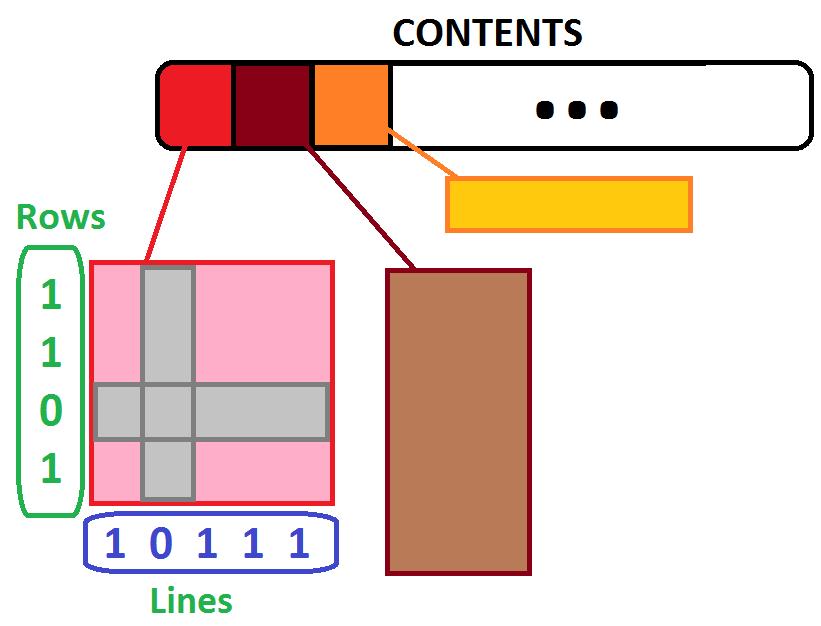
\includegraphics[scale=0.5]{matimpli.png}
  \caption{Nouvelle organisation du champ contents}
  \label{fig:phd}
\end{figure}

Ainsi, à chaque fois qu'une nouvelle matrice (à part entière) est crée, on ajoute son double vecteur de valeurs au vecteur contents et on passe en champ son index dans \texttt{contents}.

De plus, pour chaque matrice, on crée deux vecteurs \texttt{lines} et \texttt{rows} qui repèrent quelles lignes et colonnes de la matrice repérée par \texttt{index} dans \texttt{contents} sont ``actives''.

A l'origine, toutes les lignes et colonnes sont actives.

\subsection{Redéfinition des méthodes de base}

La plus grosse difficulté posée par cette construction est que l'accès à la valeur \texttt{(i,j)} de la matrice n'est plus direct: certaines lignes et colonnes sont ``désactivées''. 
Pour remédier à cela, on crée une fonction \texttt{find\_index} qui fait un parcours du vecteur de bits de maniére à trouver le bon indice.

Cela se fait en déclarant un compteur \texttt{count}, puis en faisant une boucle sur une variable \texttt{k} telle qu'à chaque itération count augmente ssi le bit d'index \texttt{k} est positif. Quand \texttt{count} > \texttt{index}, on arrête la boucle
et on récupére le \texttt{k} courant qui correspond à \texttt{real\_index + 1}. 
A partir de là, il devient très simple de redéfinir toutes le méthodes de base de Matrix en prenant soin de se rappeler que contents est maintenant un triple vecteur.

\subsection{Création de sous-matrices}

La création de sous-matrice devient très simple: on crée une copie de la matrice en question, puis on modifie les vecteurs rows et lines pour refléter le changement dans la matrice considérée.

Cela présente le grand avantage de ne pas explicitement créer un nouveau double vecteur de valeurs pour la sous-matrice. Sachant que la fonction determinant fait n! appels à la fonction submatrix les économies en temps (et mémoire) sont substantielles


\subsection{Comparaisons avec l'ancienne méthode}

Nous avons annoncé à la partie précédente que cette nouvelle façon de procéder permet de faire des économies en temps de calcul.

Pour vérifier cette affirmation, on a effectuée l'expérience suivante:

Pour $n \in \{2;4;\dots;8\}$ on génère 100 matrices aléatoires de taille $n$ et on compare les temps d'exécution de l'ancienne méthode et de la nouvelle.

Les résultats sont consignés dans le graphe suivant.

\subsection{Fuites de mémoire}

Il est important de remarquer que notre implémentation à l'aide d'un vecteur statique n'est pas sans poser de problémes de fuites mémoires.
En effet, la déclaration de nouvelles matrices dans une boucle peut causer une augmentation définitive du champ static contents.

\begin{lstlisting}
for (i=0; i < 1000; i++)
    Matrix M(10,10)
\end{lstlisting}

Avec l'ancienne implémentation, M est déclarée puis oubliée à chaque tour de boucle.

Avec notre nouvelle implémentation à l'aide du type static, la matrice de valeur stockée demeure dans contents.

Il est donc nécessaire de définir un moyen d'effacer des matrices de contents pour au moins minimiser les coûts en mémoire.

Il a donc été crée un vecteur count qui repére pour chaque matrice de valeurs stockée le nombre de matrices s'y référant. A chaque fois qu'une matrice ou sous-matrice est crée, on incrémente le compteur correspondant. On surcharge le destructeur pour qu'il décrémente ce compteur.

\subsection{Insuffisances}

Cette méthode présente cependant un gros inconvénient: les sous-matrices ainsi déclarées ont un contenu directement liée à celui des matrices mères. Si on modifie leur contenu, on modifie aussi celui de la matrice mère. et vice-versa.

Cela ne pose pas de problème dans le projet proposé puisque l'application qui en est faite agit en place sur le problème et ne modifie pas les valeurs des matrices.

En réalité, cela vient du fait que ce qu'on a voulu faire à la base est d'éviter d'expliciter des sous-matrices qu'il n'était pas nécessaire d'expliciter puisqu'on ne faisait que consulter leur valeur. Si on veut pouvoir travailler sur ces sous-matries, il faudra définir une nouvelle méthode d'extraction de sous-matrices et on ne gagnera rien par rapport à la première façon de procéder.

\section*{Conclusion}



\end{document}
